\iffalse
\author{EE24BTECH11047}
\section{ce}
\chapter{2017}
\fi
\item
The value of $M$ in the beam $ABC$ shown in the figure is such that the joint $B$ does not rotate. \\
     \begin{figure}[!ht]
    \centering
    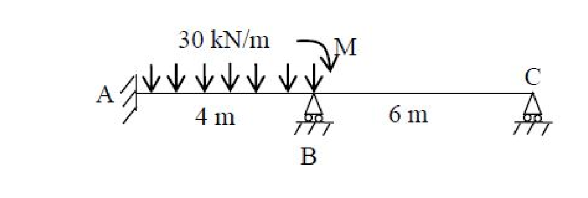
\includegraphics[width=4cm]{./GATE-yearwise/2017/figs/Q40.png}
    \end{figure}
The value of support reaction (in kN) at $B$ should be equal to.

\item
Consider the beam $ABCD$ shown in the figure.\\
     \begin{figure}[!ht]
    \centering
    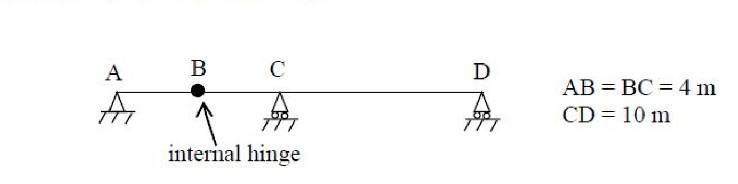
\includegraphics[width=4cm]{./GATE-yearwise/2017/figs/Q41.png}
    \end{figure}\\
For a moving concentrated load of $50 \text{ kN}$ on the beam, the magnitude of the maximum bending moment (in kN-m) obtained at the support $C$ will be equal to.

\item
Consider two axially loaded columns, namely, 1 and 2, made of a linear elastic material with Young's modulus $E = 2 \times 10^5 \text{ MPa}$, square cross-section with side $10 \text{ mm}$, and length $1 \text{ m}$. For Column 1, one end is fixed and the other end is free. For Column 2, one end is fixed and the other end is pinned. Based on Euler's theory, the ratio (up to one decimal place) of the buckling load of Column 2 to the buckling load of Column 1 is.

\item
A column is subjected to a load through a bracket as shown in the figure.
\begin{figure}[!ht]
\centering
\resizebox{0.25\textwidth}{!}{%
\begin{circuitikz}
\tikzstyle{every node}=[font=\normalsize]

\draw (0.5,10.5) to[short] (0.5,5.5);
\draw (0.5,10.5) to[short] (3,10.5);
\draw (0.5,11) to[short] (0.5,10.5);
\draw (3,11) to[short] (3,10.5);
\draw (0.5,11) to[short] (3,11);
\draw (0.5,5.5) to[short] (0.5,4.75);
\draw [->, >=Stealth] (4.25,11.25) -- (4.25,10.5);
\node [font=\normalsize] at (5,11) {P=10kN};
\draw [dashed] (3,10.5) -- (3,5.5);
\draw (0.5,5.5) to[short] (3,5.5);
\draw (0.5,4.75) to[short] (3,4.75);
\draw (3,5.5) to[short] (3,4.75);
\draw (3,10.5) to[short] (5,10.5);
\draw (3,5.5) to[short] (5,7.5);
\draw (5,10.5) to[short] (5,7.5);
\draw [dashed] (1.75,3.75) -- (1.75,12);
\draw [dashed] (0,4.25) -- (3.75,7.75);
\draw [dashed] (-0.5,7.25) -- (-0.5,7);
\draw [dashed] (1.75,10.5) -- (-0.75,7.5);
\draw [dashed] (0.75,12) -- (3,8.5);
\node [font=\normalsize] at (-0.25,8.75) {$90^{\circ}$};
\draw [dashed] (-0.75,10.75) -- (1,8);
\draw [<->, >=Stealth] (1.75,11.5) -- (4.25,11.5);
\draw [<->, >=Stealth] (-0.5,10.25) -- (1,11.75);
\node [font=\normalsize] at (0,11.25) {$10cm$};
\node [font=\normalsize] at (3,11.75) {$15cm$};
\draw [<->, >=Stealth] (-0.5,7.25) -- (0.75,5.25);
\node [font=\normalsize] at (-0.5,6.25) {$10cm$};
\draw  (1.25,9.75) circle (0.25cm);
\draw  (1.25,6.75) circle (0.25cm);
\draw  (2.5,9.75) circle (0.25cm);
\draw  (2.5,6.75) circle (0.25cm);
\node [font=\normalsize] at (0.75,10) {$1$};
\end{circuitikz}
}%

\label{fig:my_label}
\end{figure}

The resultant force (in kN, up to one decimal place) in the bolt $1$ is.

\item
A particle of mass $2 \text{ kg}$ is travelling at a velocity of $1.5 \text{ m/s}$. A force $f$(t) $= 3t^2$ N is applied to it in the direction of motion for a duration of $2$ seconds, where $t$ denotes time in seconds. The velocity (in m/s, up to one decimal place) of the particle immediately after the removal of the force is
%45-48
\item
The activity details of a project are given below:

\begin{tabular}{|c|c|c|}
\hline
Activity & Depends on & Duration (in days) \\
\hline
P & -- & 6 \\
Q & P & 15 \\
R & Q,T & 12 \\
S & R & 16 \\
T & P & 10 \\
U & Q,T & 14 \\
V & U & 16 \\
\hline
\end{tabular}\\

The estimated minimum time in days for the completion of the project will be

\item
It is proposed to drive H-piles up to a depth of 7 m at a construction site. The average surface area of the H-pile is 3 m$^2$ per meter length. The soil at the site is homogeneous sand, having an effective friction angle of 32$^\circ$. The ground water table $GWT$ is at a depth of 2 m below the ground surface. The unit weights of the soil above and below the GWT are 16 kN/m$^3$ and 19 kN/m$^3$, respectively. Assume the earth pressure coefficient, $K = 1.0$, and the angle of wall friction, $\delta = 23^\circ$. The total axial frictional resistance in kN, up to one decimal place mobilized on the pile against the driving is.

\item
The infinie sand slope shown in the figure is on the verge of sliding failure. The ground water table coincides with the ground surface. Unit weight of water $\gamma_w = 9.81 \text{kN/m}^3$.
\begin{figure}[!ht]
\centering
\resizebox{0.5\textwidth}{!}{%
\begin{circuitikz}
\tikzstyle{every node}=[font=\normalsize]

\draw [short] (-0.5,5.75) -- (4.25,7.25);
\draw [short] (-0.5,4.75) -- (4.25,6.25);
\draw [<->, >=Stealth] (-0.5,5.75) -- (-0.5,4.75);
\node [font=\normalsize] at (-0.75,5.25) {$5m$};
\draw [short] (-0.5,4.75) -- (1.5,4.75);
\node [font=\small] at (1,5) {$20^{\circ}$};
\node [font=\normalsize] at (2,6) {$\gamma_{sat}=21kN/m^3$};
\end{circuitikz}
}%

\label{fig:my_label}
\end{figure}\\
The value of the effective angle of internal friction (in degrees, up to one decimal place) of the sand is.

\item
A sluice gate used to control the flow in a horizontal channel of unit width is shown in the figure.\\
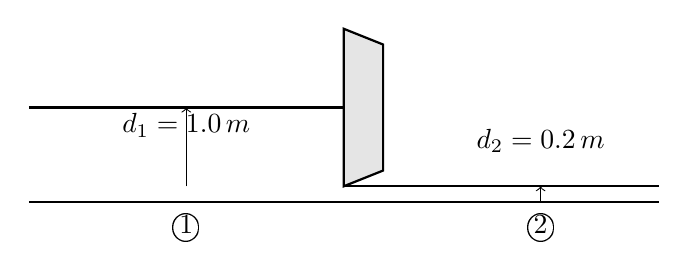
\begin{tikzpicture}

% Draw the three horizontal lines
\draw[thick] (0,1) -- (4.25,1);        % Line 1 (passes through middle of wall)
\draw[thick] (4,0) -- (8,0);    % Line 2 (passes through bottom of wall)
\draw[thick] (0,-0.2) -- (8,-0.2) ;        % Line 3 (runs from start of Line 1 to end of Line 2)

% Draw the vertical distances
\draw[->] (2,0) -- (2,1);
\node[above] at (2,0.5) {$d_1 = 1.0 \, \text{m}$};

\draw[->] (6.5,-0.2) -- (6.5,0);
\node[above] at (6.5,0.3) {$d_2 = 0.2 \, \text{m}$};

% Draw the ground labels with circles
\node[below] at (2,-0.25) {\textcircled{1}};
\node[below] at (6.5,-0.25) {\textcircled{2}};

% Draw the trapezoidal wall
\draw[thick, fill=gray!20] (4,0) -- (4,2) -- (4.5,1.8) -- (4.5,0.2) -- cycle;

\end{tikzpicture}

It is observed that the depth of flow is 1.0 m upstream of the gate, while the depth is 0.2 m downstream of the gate. Assuming a smooth flow transition across the sluice gate, i.e., without any energy loss, and the acceleration due to gravity as 10 m/s$^2$, the discharge (in m$^3$/s, up to two decimal places) passing under the sluice gate is.
%49-52
\item
Water flows through a $90^{\circ}$ bend in a horizontal plane as depicted in Figure.\\
     \begin{figure}[!ht]
    \centering
    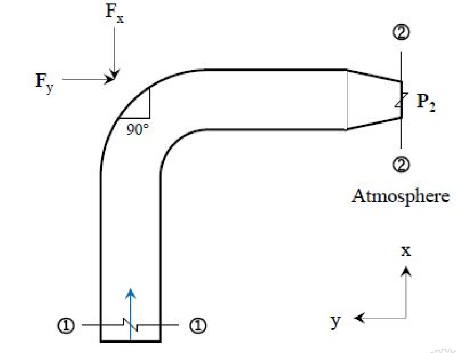
\includegraphics[width=2.5cm]{./GATE-yearwise/2017/figs/Q49.png}
    \end{figure}

The pressure at Section 1, $P_1 = 140 \text{ kPa}$, and the inlet diameter at Section 1 is $\frac{27}{\sqrt{\pi}} \text{ cm}$. The nozzle diameter at Section 2 is $\frac{18(14)}{\sqrt{\pi}} \text{ cm}$. \\
Assuming acceleration due to gravity, $g = 10 \text{ m/s}^2$, and neglecting the weights of both the pipe segment and water, as well as friction across the bend, calculate the magnitude of the force (in kN up to two decimal places) required to hold the pipe section.

\item
A consolidated undrained (CU) triaxial compression test is conducted on normally consolidated clay at a confining pressure of $100 \text{ kPa}$. The deviator stress at failure is $80 \text{ kPa}$ and the pore-water pressure at failure is $50 \text{ kPa}$. Calculate the effective angle of internal friction (in degrees , up to one decimal place) of the soil.

\item
An effective rainfall of 2-hour duration produces a flood hydrograph with a peak of $200 \text{ m}^3/\text{s}$. The base flow of the hydrograph is $20 \text{ m}^3/\text{s}$. The spatial average rainfall in the watershed is $2 \text{ cm}$ and the average loss rate is $0.4 \text{ cm/hour}$. Calculate the peak of the 2-hour unit hydrograph in ${m}^3$/s, up to one decimal place.

\item
Given four sources with noise levels of $60 \text{ dB}$, $69 \text{ dB}$, $70 \text{ dB}$, and $79 \text{ dB}$, calculate the equivalent sound power level in dB of the four sources.

t
